\chapter{The LAGUNA-LBNO Near Detector Concept}
The ND is a crucial instrument for neutrino oscillation measurements. It provides details of the unoscillated flux, including measurements of the neutrino beam direction and profile. Measurements of the energy spectrum and electron neutrino contamination are also monitored with the ND. The systematics and accuracy of the ND can constrain the precision of the whole experiment, so great care must be taken in the design and construction of such a detector. With little neutrino cross sectional data in the medium energy regime, the ND can also function to perform such precision measurements. 

With LAGUNA-LBNO being a feasibility study, there is no concrete design of the ND. Liverpool University was heavily involved with the ND design since the formation of the LAGUNA-LBNO collaboration and proposed the initial detector design and technology. With collaborations within the LAGUNA-LBNO project this design was refined and investigated, with Liverpool the driving force in the design. I was personally involved with all ND efforts and represented the University of Liverpool within the collaboration. For the LAGUNA-LBNO experiment we propose a Gas Argon (GAr) Time Projection Chamber (TPC) with surrounding scintillator layers and this chapter hopes to introduce the overall concept of the detector with a discussion on the requirements imposed on the ND. 

\vspace{5mm}
\section{Requirements}
The ND must be able to:
\begin{itemize}
	\item{\textbf{Measure the absolute neutrino flux:}} The Near/Far ratio is used to extrapolate the flux at the ND to the FD without oscillation. Many factors are required for an accurate measurement of this, with descriptions of the beam profile, direction and neutrino energies of big concern.
%This is important to understand if the beam tuning has been correctly established.  
	\item{\textbf{Monitor the beam contamination:}} It is important to know the electron neutrino contamination of the beam, as an accurate understanding of the beam composition reduces the uncertainty on oscillation measurements in the FD. The electron contamination of the beam is a large background for electron neutrino appearance measurements and must be well understood. Using a magnetised ND will allow for charge identification and will discriminate between charged leptons produced from CC interactions.
	\item{\textbf{Perform cross sectional measurements:}} With a poor understanding of neutrino cross sections on different materials, it is important for present and future experiments to understand their interactions better. There is a need within the neutrino community to perform accurate cross sectional measurements in the medium energy regime (several GeV). Without new and improved measurements then experiments will be limited by these systematical uncertainties. The FD cannot perform such measurements due to neutrino oscillations and hence must be performed at the ND.
\end{itemize}

\section{The Detector Design}
As a result of the requirements imposed, the ND must poses the ability to reconstruct the energy of the neutrino, the interaction point (vertex) and flavour of the neutrino. In order to perform this a multilayer detector is proposed, consisting of two main sections, the TPC and the scintillator layer (TAS):
\begin{itemize}
	\item{\textbf{Primary Detector - Time Projection Chamber (TPC):}}
	\begin{itemize}
		\item Vertex location and tracking
		\item Perform momentum measurements on charged particles
		\item Charged particle identification
	\end{itemize}
	\item{\textbf{Secondary Layer - Totally Active Scintillator (TAS):}}
	\begin{itemize}
		\item Additional particle identification
		\item Neutral particle energy reconstruction, $\pi^{0}$'s and $\gamma$'s
	\end{itemize}
\end{itemize}
These sub detectors are discussed sequentially.

\section{The Time Projection Chamber} 
Both beam options offer neutrinos with a broad energy spectrum, peaking between 1-7 GeV, and in this energy regime DIS events dominate. In order to deal with the high multiplicities of such interactions the primary detector must be able to resolve and reconstruct multiple tracks. A clear candidate for the detection medium in the ND is argon, primarily due to its ability to deal with high multiplicity events with very good position reconstruction. It is also important for the target material to match that of the FD to reduce systematical uncertainties in oscillation measurements, avoiding nuclear effects and uncertainties in material cross sections. With the FD chosen to be of either GLACIER or LENA technology then argon and carbon are likely candidates for the ND target material. Considerable favour has fallen to the former technology in the LAGUNA-LBNO study and coupled with the many benefits of using noble gases as detection media, argon is implemented as the primary detector medium. 
 
The FD of GLACIER technology comprises of LAr with a GAr amplification phase, operating in both charge and light collection modes. However such a design is not recommended for the ND with GAr used as the sole medium. Argon is liquid below 87.26 K and hence requires cryogenics to maintain it in this state. Such additional instrumentation increases costs and can require cumbersome extra infrastructure. Using GAr does not require the same instrumentation and avoids the difficulties cryogenics introduces. Such comparisons are albeit rather negligible when considering the difference in densities however. The difference in density between gas and liquid phases results in a factor of $\sim$1000 difference, with LAr at 1.4 gcm$^{-3}$ and GAr at 1.7 $\times$ 10$^{-3}$ gcm$^{-3}$ (at boiling point). With the ND far closer to the beam origin the neutrino beam is far more intense at the ND, $\sim$8 $\times$ 10$^{6}$ larger, assuming an inverse square law dependance. The difference in densities is then crucial when considering detector performance, as pileup becomes a serious issue, with the event rate scaling proportionally to the density. The detector event rate per unit volume can then be tailored to the desired rate by altering the GAr pressure. Studies within LAGUNA-LBNO have shown that tracking in GAr (20 bar) is successful and can be superior to liquid \cite{lbnoInternalCurioni}, as can be seen in figure \ref{fig:GArVsLAr}.

\begin{figure}[hbtp]
	\begin{center}
		\includegraphics[width=150mm]{Chapter3/figures/liquid-gas-argon1-1.png}
	\caption{Comparing quasi-elastic charged current interactions in LAr (upper) and 20 bar GAr (lower). The three protons from the interaction vertex are apparent in the GAr TPC, but cannot be resolved in the LAr. Image taken from \cite{lbnoNDTechNote}.}
	\label{fig:GArVsLAr}
	\end{center}
\end{figure}

%Avoiding LAr also results in the omission of cryogenics, as Argon is liquid below 87.26K and hence requires significant cooling to maintain it in this state. Cryogenics can increase costs while also introducing extra implementation and technical difficulties.  

The most common and powerful technology utilising argon as its medium is the TPC, this follows suit from the FD design. A 2 $\times$ 2 $\times$ 2 m$^{3}$ GAr TPC is implemented for the ND primary target, pressurised to 20 bar. At this pressure the density of argon is 0.035 gcm$^{-3}$, yielding a detector mass of 280 kg. This design is loosely based on the T2K ND, ND280 \cite{internalT2K}, where three TPCs, each of volume 1808 $\times$ 2230 $\times$ 854 mm, are used as the sensitive volume in the detector. The proposed LAGUNA-LBNO ND is smaller, largely due to restrictions on the pressure vessel, which is discussed later. 

%The TPC performs well at measuring $dE/dx$ which can provide good discrimination between electrons and muons.

\subsection{Momentum Measurements}
The majority of muons generated in the TPC will leave the volume, as a peak energy $\sim$3 GeV $\mu^{-}$ will travel $\sim$3 m in argon. A magnetised TPC will allow the measurement of charged particles momentum given a large enough sagitta measurement. When a charged particle passes through the magnetic field, $\boldsymbol{B}$ = (0,0,$B_{z}$), it will cause a curved trajectory, ignoring scattering, as shown in figure \ref{fig:sagitta}. 
\begin{figure}[hbtp]
	\begin{center}
		\includegraphics[width=100mm]{Chapter3/figures/sagittaDrawing.png}
	\caption{An illustration showing a charged particle passing through a magnetic field $\boldsymbol{B}$ at a velocity $\boldsymbol{v}$ following curvature parametrised by the sagitta $s$, of radius $r$, and of track length $L$.  }
	\label{fig:sagitta}
	\end{center}
\end{figure}
The sagitta, $s$, is given in terms of the radius of curvature, $r$ ,and track length, $l$, in equation \ref{eq:sagitta1}. To a good approximation ($s \ll l$) the strength of the magnetic field strength can be estimated as equation \ref{eq:magFieldSagitta} in terms of the transverse momentum, $p^{trans} = \sqrt{p^{2}_{x} + p^{2}_{y}}$.
\begin{equation}
	s = r - \sqrt{r^{2} - (l/2)^{2}} \simeq \frac{l^{2}}{8r}
	\label{eq:sagitta1}
\end{equation}
\begin{equation}
	B_{z} = \frac{8sp^{trans}}{el^{2}} = \frac{26.7s[m] p^{trans} [GeV/c]}{l^{2}[m^{2}]}
	\label{eq:magFieldSagitta}
\end{equation}
Thus an estimation of the magnetic field required can be established by determination of an adequate measurement of the sagitta. Based on the T2K ND280 detector design the space point resolution of the TPC is approximately 300 $\mu$m \cite{internalT2K}, which translates to roughly the same value for $\delta s$ given $N_{p}$ = 5 equidistantly spaced points per track using the Gluckstern formula \cite{GlucksternFormula} as shown in equation \ref{eq:GlucksternEquation}. Here we consider uncertainties on the magnetic field and the track lengths to be negligible. Using this value and assuming a $\delta p/p$ $\sim$ 5\% provides $s \sim$ 6 mm. Given a 3 GeV/c muon, with the majority of its momentum in the transverse direction, leaving a track length of $\sim$1 m in the TPC, translates to a magnetic field strength of $\sim$0.5 T.

\begin{equation}
	\delta p^{trans}/p^{trans} \sim \delta s/s = \frac{\sigma_{xy}p^{trans}}{8s}\sqrt{\frac{720}{N_{p} + 4}}
	\label{eq:GlucksternEquation}
\end{equation}

\section{Total Active Scintillator}
The TAS will instrument the volume outside the TPC. It is to complement the TPC measurements and is envisaged to contribute to the reconstruction of neutrino interactions in the TPC. Its function is primarily to reconstruct neutral particles such as photons, with many originating from the decay of neutral pions. Its secondary function is to involve cross-section measurements for neutrino interactions in plastic.

To define the amount of matter traversed by high energy photons and electrons for interactions relating to pair production and Bremsstrahlung respectively, the radiation length, $X_{0}$, is used. It is usually measured in gcm$^{-2}$ and can be interpreted as the mean distance at which the electron has lost all but 1/$e$ of its original energy by Bremsstrahlung and 7/9 of the mean free path for pair production of photons. The radiation length is given by equation \ref{eq:radiationLength} which originates from fits to experimental data \cite{radiationLengthsBook}.

\begin{equation}
	X_{0} = \frac{716.4 [\textnormal{gcm}^{-2}] A}{Z(Z+1) \textnormal{ln}(287 / \sqrt{Z})}
	\label{eq:radiationLength}
\end{equation}
Here A and Z are the atomic mass number and proton number respectively. When considering a composition of materials or chemicals, then a total radiation length can be approximated by equation \ref{eq:radiationLengthCombined}. Here $w_{i}$ is the weight fraction of element $i$ in the material and $X_{i}$ is the radiation length of element $i$.

\begin{equation}
	\frac{1}{X_{0}} = \sum_{i} \frac{w_{i}}{X_{i}}
	\label{eq:radiationLengthCombined}
\end{equation}
Plastic scintillator bars are proposed with Wave Length Shifting (WLS) fibres and compact Multi Pixel Photon Counters (MPPCs) to readout the scintillation light. Once again this design follows from the T2K ND280 scintillator detector implementation, which is well established technology. A chemical composition of C$_{5}$O$_{2}$H$_{8}$ is assumed for the scintillator bars and the resulting radiation length of this, along with that of $^{12}$C,$^{16}$O and $^{1}$H individually, is shown in table \ref{tab:radiationLengths}. The bars themselves can be seen in figure \ref{fig:scintBars} and have dimensions of 10 $\times$ 10 $\times$ 900 mm$^{3}$.

\begin{table}
\begin{center}
  \begin{tabular}{l*{4}{c}r}
  \hline
  \textbf{Material} & \textbf{A} & \textbf{Z} & $\boldsymbol{X_{0}}$ \textbf{[gcm$^{-2}$]} \\
  \hline
  \hline
  Hydrogen & 1 & 1 & 63.3 \\
  Carbon & 12 & 6 & 43.0 \\
  Oxygen & 16 & 8 & 34.5 \\
  C$_{5}$O$_{2}$H$_{8}$ & - & - & 40.8 \\
  \hline
  \end{tabular}
      \caption{The radiation lengths, $X_{0}$, for $^{1}_{1}$H, $^{12}_{6}$C, $^{16}_{8}$O and C$_{5}$O$_{2}$H$_{8}$. The results are calculated from the use of equation \ref{eq:radiationLength} and equation \ref{eq:radiationLengthCombined}.}
    \label{tab:radiationLengths}
\end{center}
    \end{table}

\begin{figure}[htbp]
	\begin{center}
		\includegraphics[width=120mm]{Chapter3/figures/scintBars.png}
	\caption{The proposed design of the scintillation bars used in the ND. Image taken from \cite{lbnoInternal}.}
	\label{fig:scintBars}
	\end{center}
\end{figure}
The MPPCs to be used for scintillation light readout are manufactured by Hamamatsu and customised for the T2K experiment. Each MPPC consists of 667 pixels with a total sensitive area of 1.3 $\times$ 1.3 mm$^{2}$ and can be seen in figure \ref{fig:mppc}. The use of MPPCs, as opposed to PMTs, is due to the large size of PMTs, typically $\sim$10 cm diameter, making it very difficult to integrate two for each scintillator bar but also because PMTs cannot operate in magnetic fields. MPPCs however can operate perfectly fine in magnetic fields and require much lower operation voltages, 70 V, compared to 2 kV for PMTs. MPPCs rely on the detection of photons via the photoelectric effect, as a photon after being wavelength shifted will reach a pixel and generate photoelectrons. The subsequent production of further electrons via an avalanche, amplifies the signal, as the amount of electron-hole pairs increases the voltage drops across the diode. If the voltage drop is over the set threshold then a signal is generated for the pixel. Each pixel is then a binary system, with the number of pixels triggered proportional to the number of photons incident on the MPPC. 
\begin{figure}[htbp]
	\begin{center}
		\includegraphics[width=49mm]{Chapter3/figures/mppc1.png}
		\includegraphics[width=50mm]{Chapter3/figures/mppc2.png}
	\caption{The MPPC proposed for use within the scintillator bars. Image taken from \cite{lbnoEoI}.}
	\label{fig:mppc}
	\end{center}
\end{figure}

\section{Other Detector Components}
The TPC imposes additional instrumentation of the detector, mainly a pressure vessel required for the GAr TPC and a magnet to perform momentum measurements and charge identification.
\subsection{Pressure Vessel}
To maintain 2 MPa of pressurised GAr in the TPC a pressure vessel is required. Pressure vessels are commonly of cylindrical shape, other than a sphere this shape provides the best structural support. The material composition of the vessel is aluminium. The vessel has an outer diameter of 5 m, a length of 5 m, and is of thickness 50 mm. With little engineering focus on the pressure vessel the dimensions are approximate with an estimated internal volume of $\sim$90 m$^{3}$. 

Due to the pressure vessel the scintillator bars will need to be placed inside the vessel to provide continuity in the detector and avoid neutrino interactions within the vessel contaminating the signal. This will cause particular engineering difficulties but would not prove impossible to implement.

\subsection{Magnet}
With no studies performed on the magnet design and no engineering effort established for its development, a very simple implementation is considered for the ND. It is proposed that a dipole magnet is implemented which is capable of providing a magnetic field strength of 0.5 T. Such a magnet will surround the whole detector assembly to enable momentum measurements in the TPC. The magnetic field must be parallel to the drift direction for charge carriers in the TPC to avoid $\textbf{B} \times \textbf{v}$ cross effects from the Lorentz Force. 

%No study focused on the magnet design has been conducted within the LAGUNA-LBNO collaboration. 
 
\section{Location}
The position of the ND from the beam target is not a trivial matter. Several factors govern its distance from the target: cost, engineering and particle rates. Due to cost restrictions and engineering difficulties an upper bound of 1000 m from the target is set. At this distance excavation to a depth of -220 m is needed and becomes unfeasible for depths greater than this. Beam requirements also cause heavy restrictions on the ND placement, with muons originating from the beam, decay pipe and horns creating extremely large muons rates to the ND. The reduction of this rate can be controlled by increasing the distance between the ND and the target or deflecting them via use of a magnet. The latter would require high magnetic fields and is too expensive to be considered, with it far more viable to increase the target ND distance. Due to costs the ND position is at 800 m from the target, at this distance a rate of $\sim$2.5 $\mu$/m$^{2}$/10$^{13}$ can be expected based on beam simulation studies \cite{lbnoInternal}.

%Figure \ref{fig:muonsFromBeamFlux} shows initial results from a beam simulation of the expected muon flux at certain distances from the beam target, with rates at 800 m at $\sim$10 $\mu$/cm$^{2}$/7$\times$10$^{13}$ p.o.t. This can be reduced by increasing the distance between the ND and the target or deflecting them via use of a magnet. Recent studies from the beam group \cite{lbnoInternal} have reduced this initial figure considerably at 800 m to $\sim$2.5 $\mu$/m$^{2}$/10$^{13}$ by introducing.... however the reduction of this rate further seems a difficult task and a lower bound of 800 m from the target is incurred for the ND placement. The minimum distance of 800 m is favourable for the ND placement mainly due to costs.
%\begin{figure}[htbp]
%	\begin{center}
%		\includegraphics[width=130mm]{Chapter3/figures/muonsFromBeam.pdf}
%		\caption{}
%		\label{fig:muonsFromBeamFlux}
%	\end{center}
%\end{figure}

\section{Neutrino Flux at the Near Detector}
The neutrino flux is optimised for the FD, not the ND, and so the flux may vary significantly from what is expected at the FD. The ND is an on axis detector in order to cover a wide energy range. Some other long baseline experiments such as T2K, use off-axis beam placement to tune the neutrino energies to narrower energy regime, however this is not the case for LAGUNA-LBNO. 

Simulations have been conducted by the beam group within the LAGUNA-LBNO study to estimate the neutrino flux at the ND. Using FLUKA\cite{fluka}, the expected 2 flavour ($\mu$ and e flavour) neutrino flux with their antiparticle counterparts expected at the ND is determined in the energy range 0 - 30 GeV. Above this energy the neutrino flux is negligible and can be approximated as zero. Considering the two beam options, 50 and 400 GeV beam, both are shown in figure \ref{fig:neutrinoFluxND} for positive horn ($\nu_{\mu}$ run) and negative horn ($\bar{\nu}_{\mu}$ run) focusing. 
\begin{figure}[htbp]
	\begin{center}
		\includegraphics[width=74mm]{Chapter3/figures/400_PF_800m_2o5mRadius_allFlav_combined.pdf}
		\includegraphics[width=74mm]{Chapter3/figures/400_NF_800m_2o5mRadius_allFlav_combined.pdf}
		\includegraphics[width=74mm]{Chapter3/figures/50_PF_800m_2o5mRadius_allFlav_combined.pdf}
		\includegraphics[width=74mm]{Chapter3/figures/50_NF_800m_2o5mRadius_allFlav_combined.pdf}
		\caption{Expected neutrino flux as a function of neutrino energy for positive focusing (left) and negative focusing (right) for beam options of 400 GeV (upper) and 50 GeV (lower). These plots show a 2.5 m radius cut selection, covering an area of 19.6 m at 800 m from the beam target. Errors bar show statistical error of $\pm$ 1$\sigma$. }
		\label{fig:neutrinoFluxND}
	\end{center}
\end{figure}

The flux at the ND does not follow a simple inverse square law ($1/r^{2}$) due to the finite dimensions of the decay pipe, as neutrinos are generated at various positions in this pipe. However for very good approximation this can be used for the FD as the distance is so great, the source can be seen as point like. This can cause problems for the extrapolation of the neutrino flux to the FD given information only on the ND flux. To give a comparison of this between ND placements, the $\nu_{\mu}$ expected flux at the ND for the 400 GeV PF is shown for 800, 900 and 1000 m distances from the beam target in figure \ref{fig:fluxDistances}. The integrated flux at distances from 800 m to 1000 m deviates slightly from the extrapolated flux following an inverse square law as figure \ref{fig:fluxDistanceValues} shows.
\begin{figure}[htbp]
	\begin{center}
		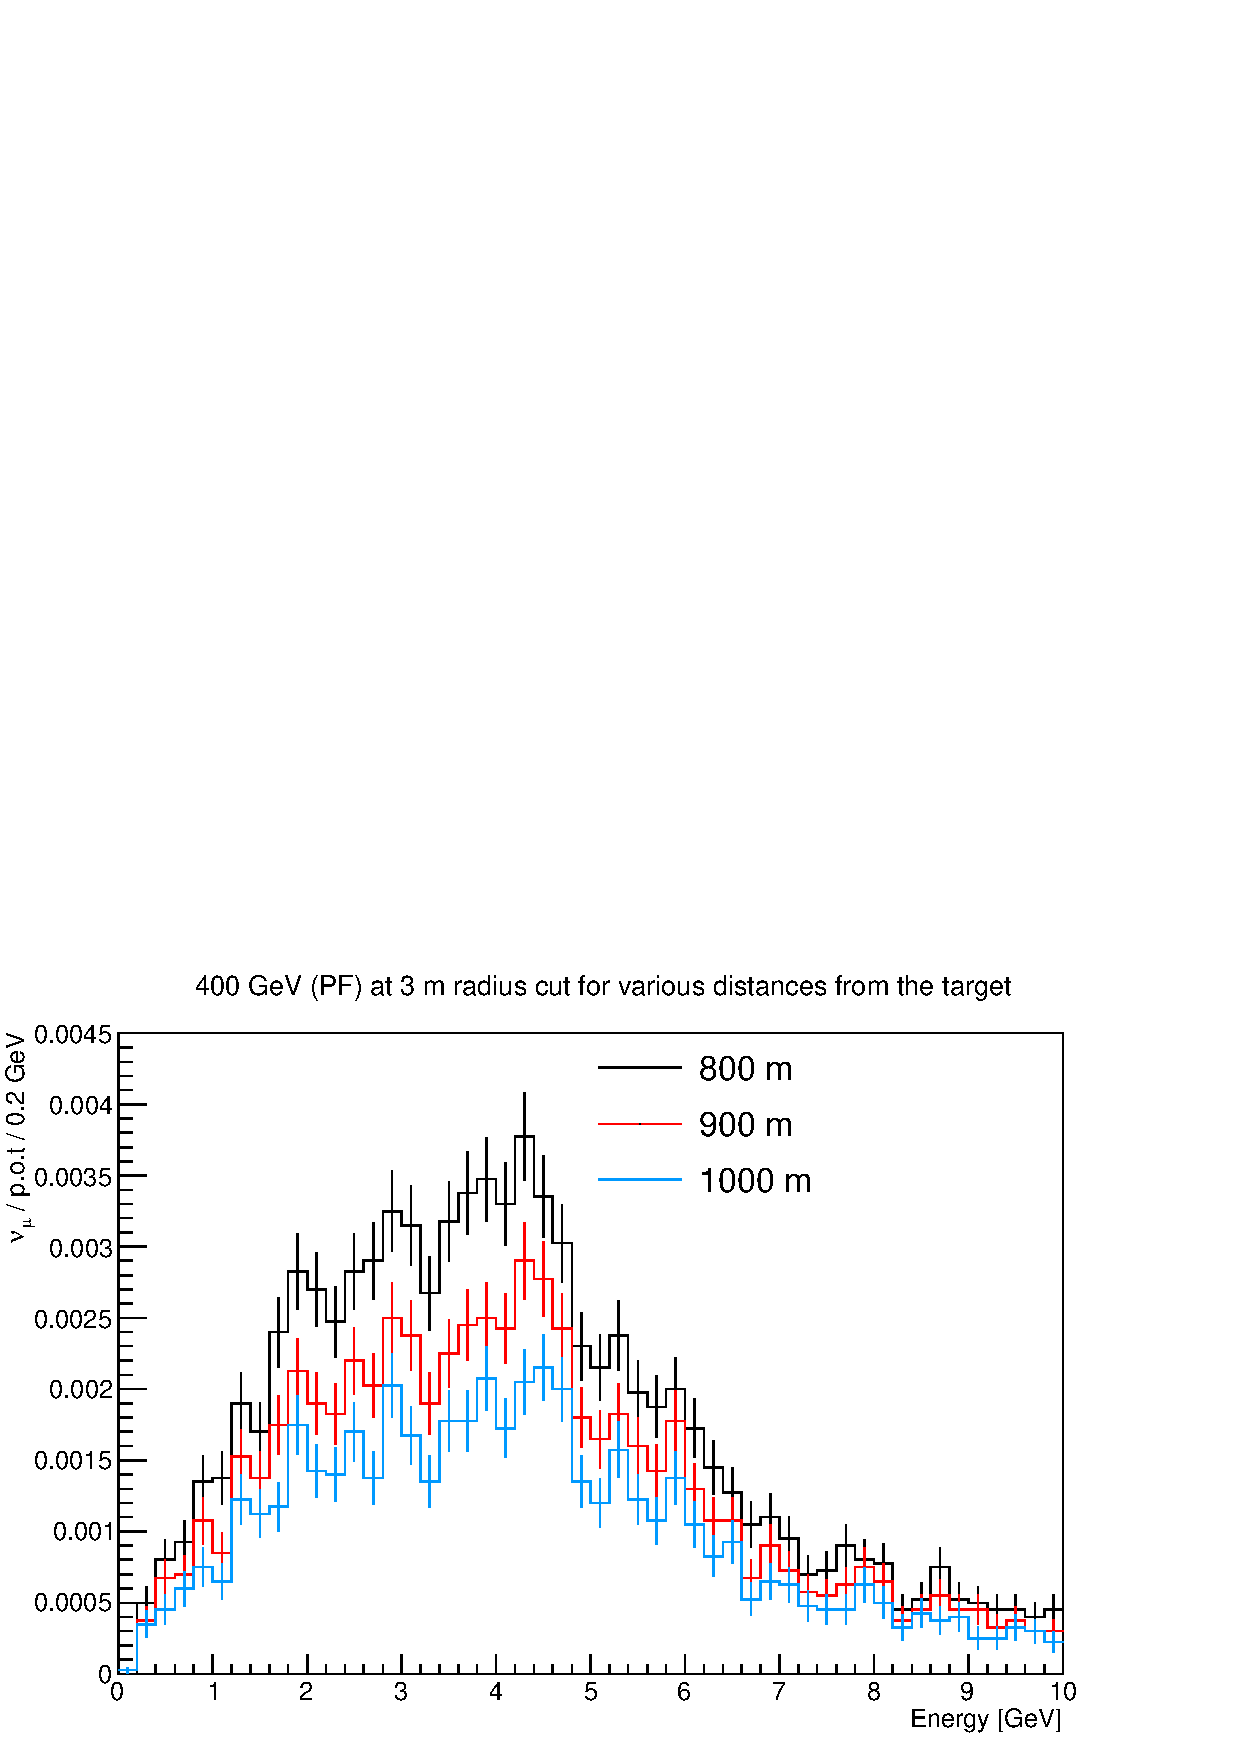
\includegraphics[width=100mm]{Chapter3/figures/400_PF_numu_distancePlot.pdf}
		\caption{Expected neutrino flux as a function of neutrino energy for the 400 GeV beam in positive focusing mode. These plots show a 2.5 m radius cut selection, covering an area of 19.6 m at 800 m from the beam target. Errors bar show statistical error of $\pm$ 1$\sigma$. }
		\label{fig:fluxDistances}
	\end{center}
\end{figure}

\begin{figure}[htbp]
\begin{center}
 	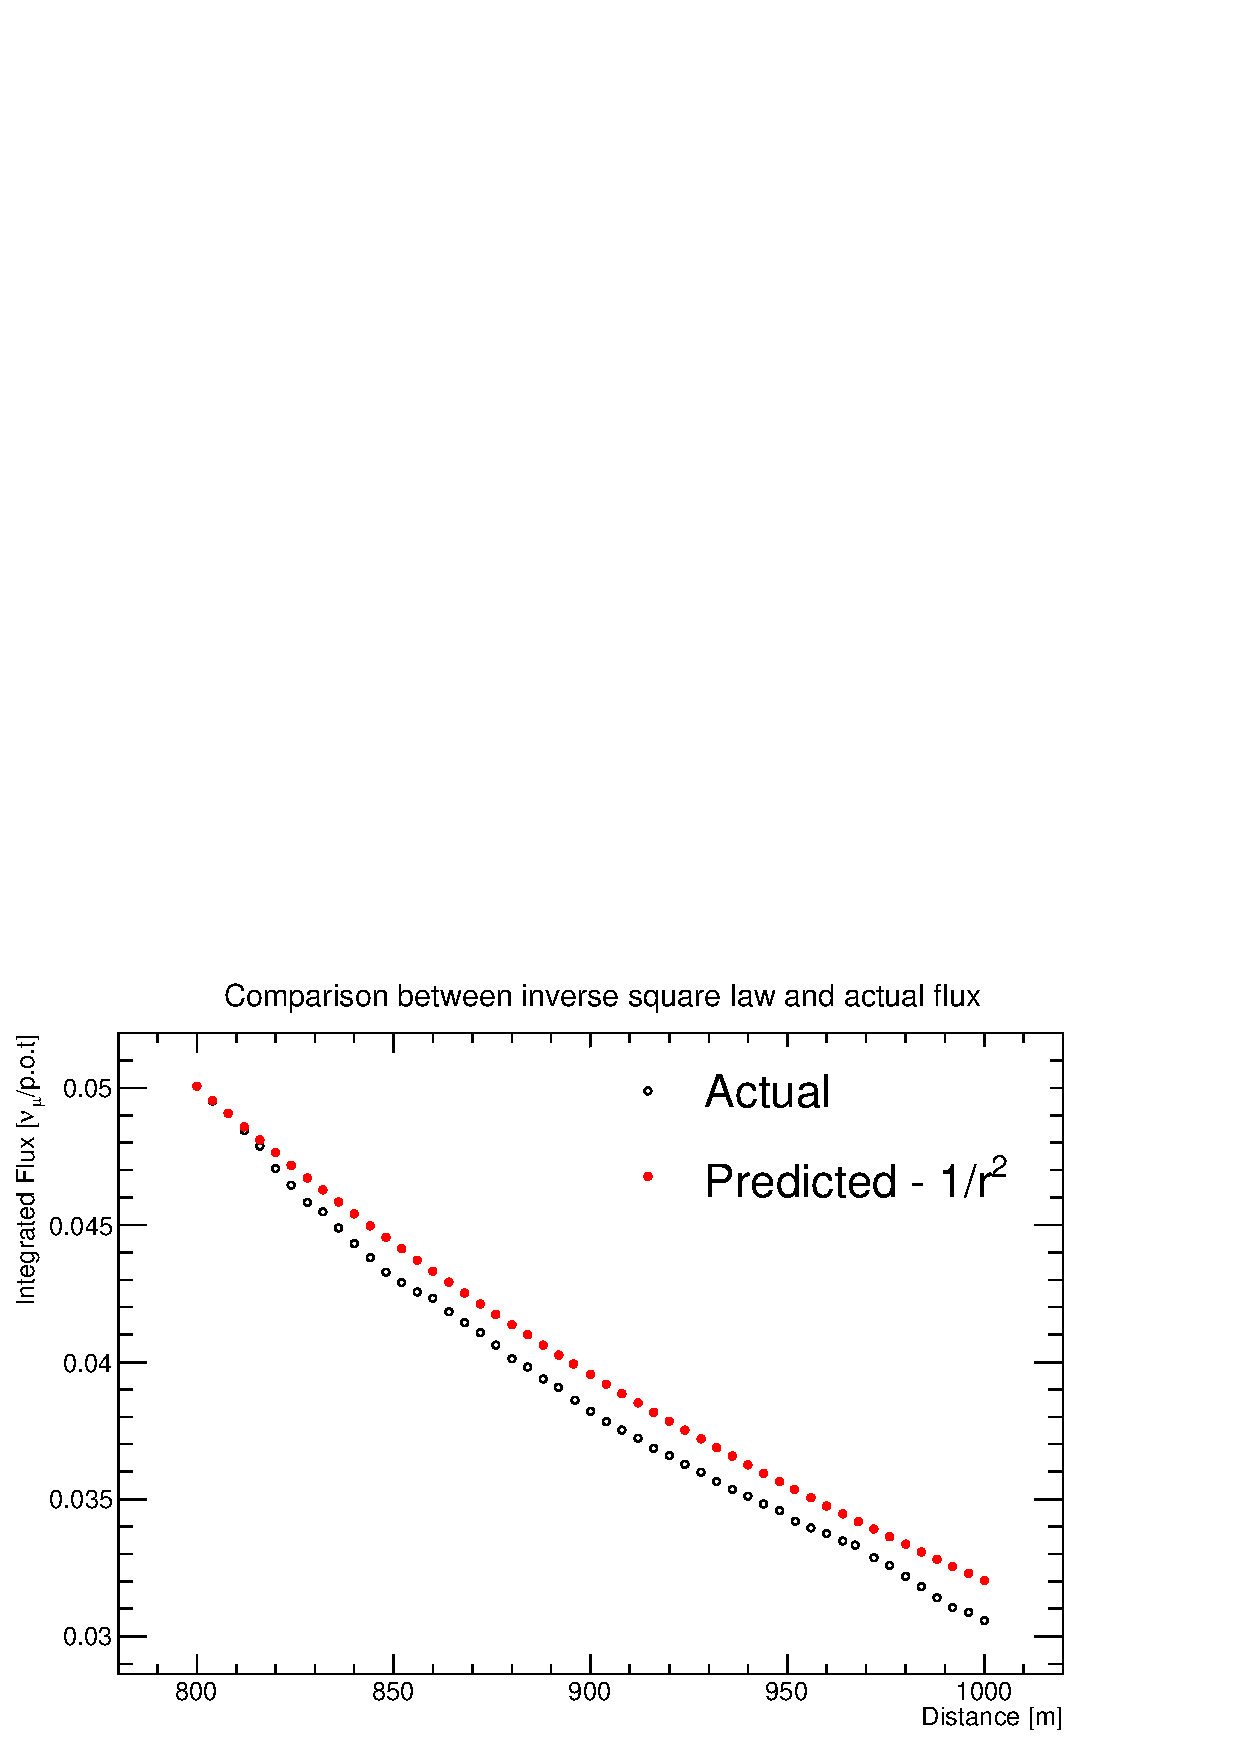
\includegraphics[width=100mm]{Chapter3/figures/400_PF_numu_inverseSquareLaw.pdf}
      \caption{The comparison between actual integrated flux (0 to 10 GeV) at distances from 800 to 1000 m from the beam target to the predicted flux extrapolated from the 800 m value, based on a 1/$r^{2}$ law. Results based on 400 GeV PF beam option only.}
    \label{fig:fluxDistanceValues}
\end{center}
\end{figure}

The neutrino flux is vastly reduced and its spectrum is broadened upon decreasing the radius cut selection. Figure \ref{fig:numuFluxRadius} shows the $\nu_{\mu}$ flux at 800 m from the target incident on circular areas of radii 1.5, 2.5, 10.0 and 30.0 m. The first two cuts are of particular significance to the ND, a radius cut of 1.5 m (7.1 m$^{2}$ area) covers the TPC and at 2.5 m (19.6 m$^{2}$ area) covers the whole ND vessel. The larger radius cuts are relevant for understanding background neutrino interactions in the surrounding detector environment and the rock.

\begin{figure}[htbp]
\begin{center}
 	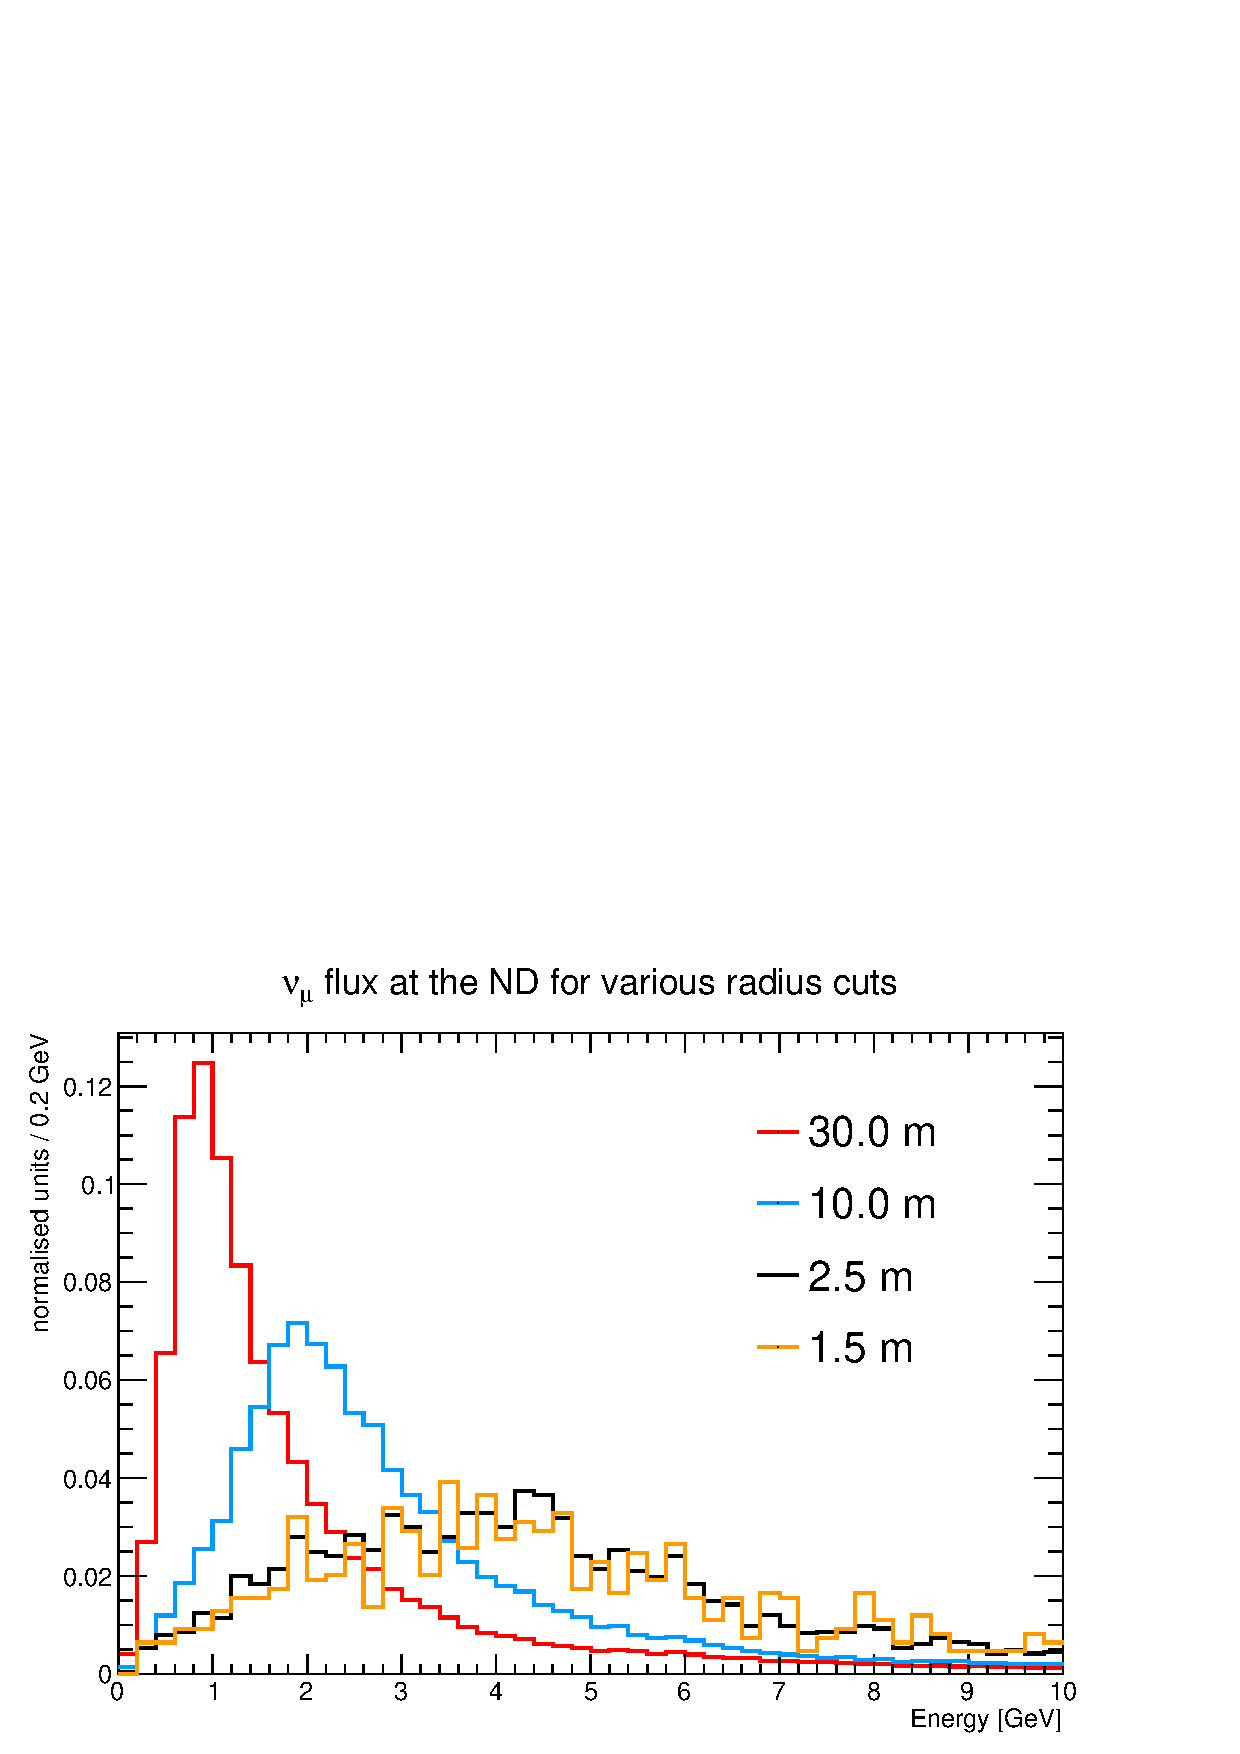
\includegraphics[width=100mm]{Chapter3/figures/400GeV_PF_numuRadiusCuts.pdf}
      \caption{The expected muon neutrino flux at 800 m from the target for radius selections of 1.5 m in orange, 2.5 m in black, 10 m in blue and 30 m in red. Each radius selection is normalised to the number of entries such that the integral is equal to 1, scale factors of 2.8, 22.4 and 59.2 are used for 10, 2.5 and 1.5 m radii respectively to compare rates with the 30 m radius cut. Results based on 400 GeV PF beam option only.}
    \label{fig:numuFluxRadius}
\end{center}
\end{figure}

The electron neutrino contamination of the beam as a function of cumulative radius selection can be seen on the left of figure \ref{fig:nueContamination}. A radius selection of $\sim$1.5 m covers the TPC and at this radius the electron neutrino contamination, $\alpha_{\nu_{e}}^{cont}$ = ($\nu_{e} + \bar{\nu}_{e}$)/($\nu_{\mu} + \bar{\nu}_{\mu} + \nu_{e} + \bar{\nu}_{e}$) is 0.7$^{+0.4}_{-0.3}$\% (stat error only). The statistical errors are rather large for the electron neutrino contamination due to the limited statistics of the beam flux file for the 1.5 m radius selection. The generation of larger statistics is computational intensive and is done externally by the LAGUNA-LBNO beam group, given their time constraints, we are subsequently limited to these low statistics. As the main focus of the studies in this thesis are concerned with the muon neutrino interactions primarily, it is not an issue however. Increasing the radius selection to 30 m increases the statistics of $\nu_{e}$ and $\bar{\nu}_{e}$ by a factor of 165 (from 6 to 990 $\nu_{e}$ + $\bar{\nu}_{e}$ passing the radius selection) and how this contamination varies with energy selection can be seen in the right of figure \ref{fig:nueContamination}. The inclusion of the $\bar{\nu}_{\mu}$ contamination is shown in figure \ref{fig:nueAndNuMuBarContamination}.

\begin{figure}[htbp]
\begin{center}
 	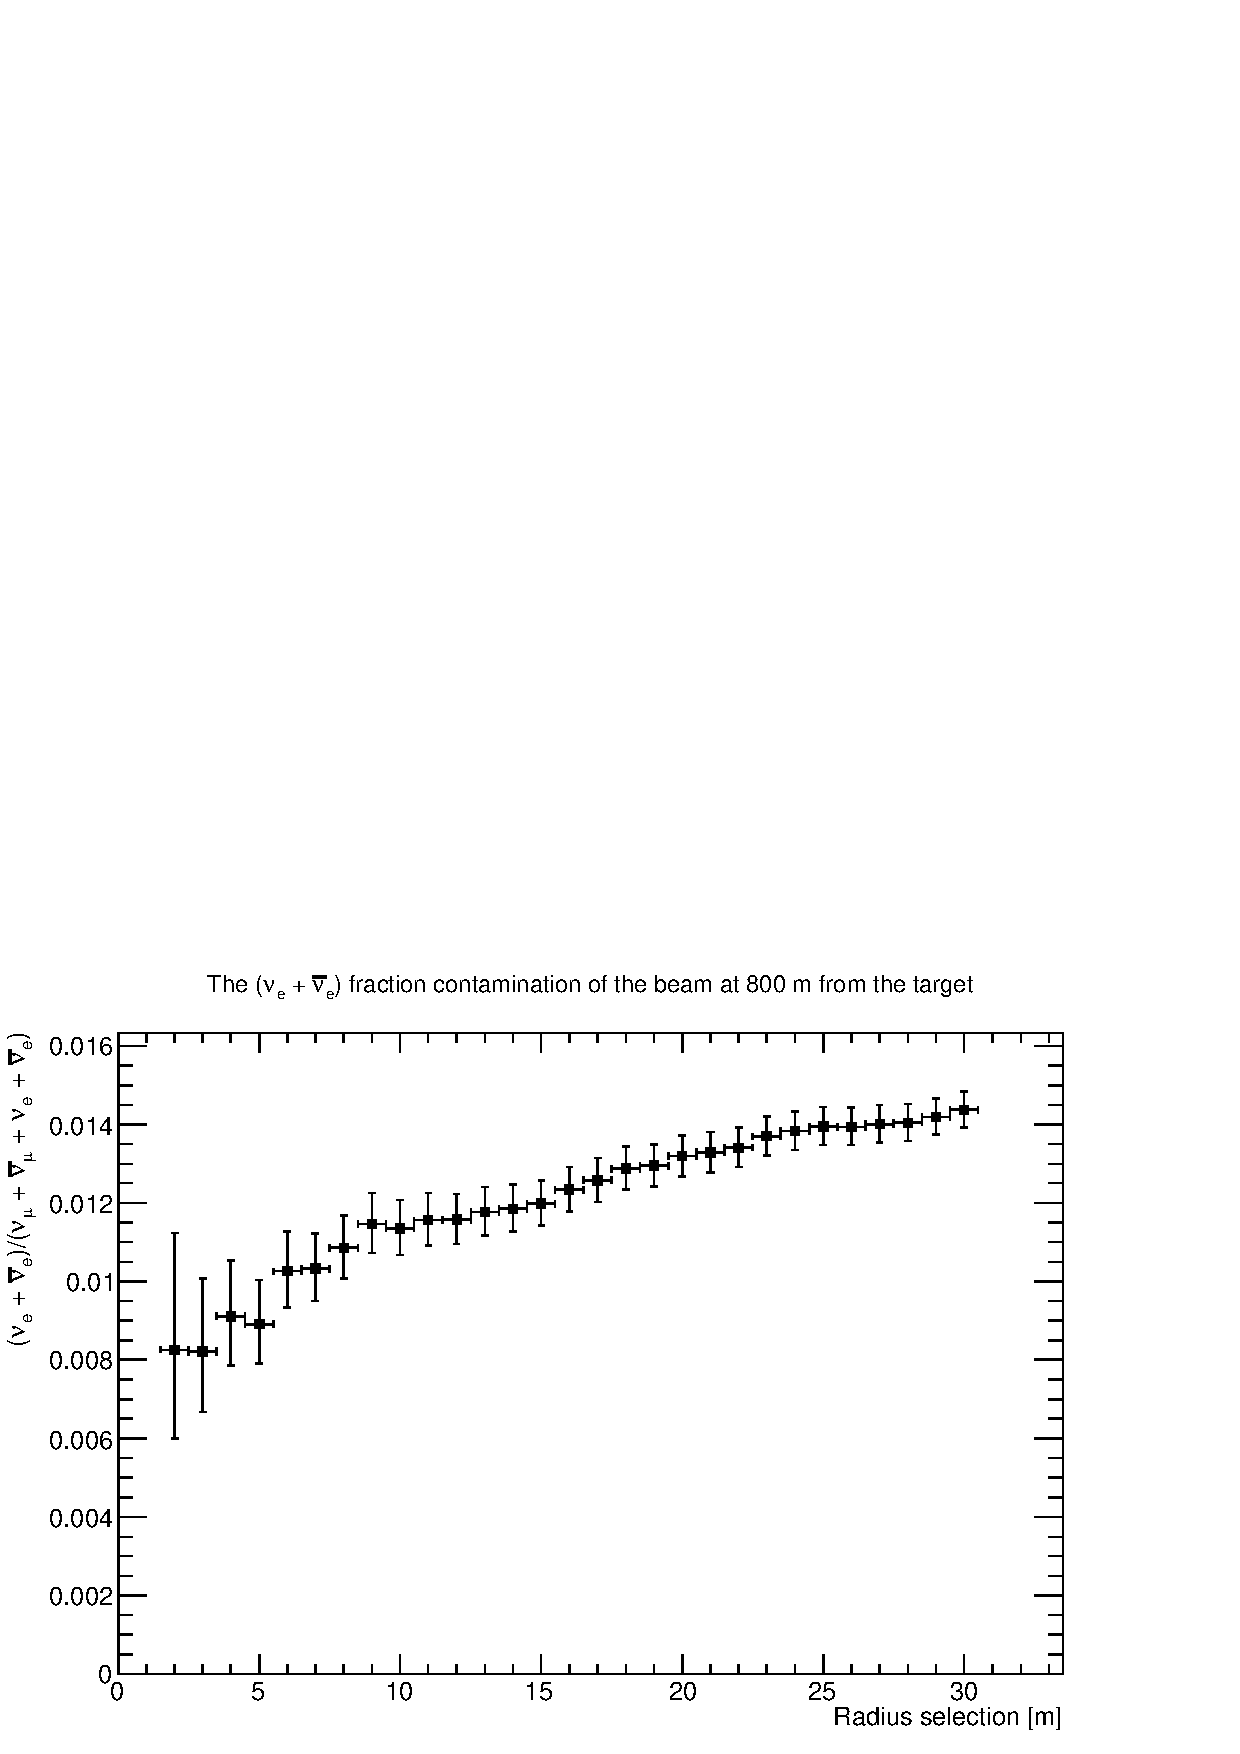
\includegraphics[width=120mm]{Chapter3/figures/400GeV_PF_nueAndNueBarRatio_RadiusCuts.pdf}
 	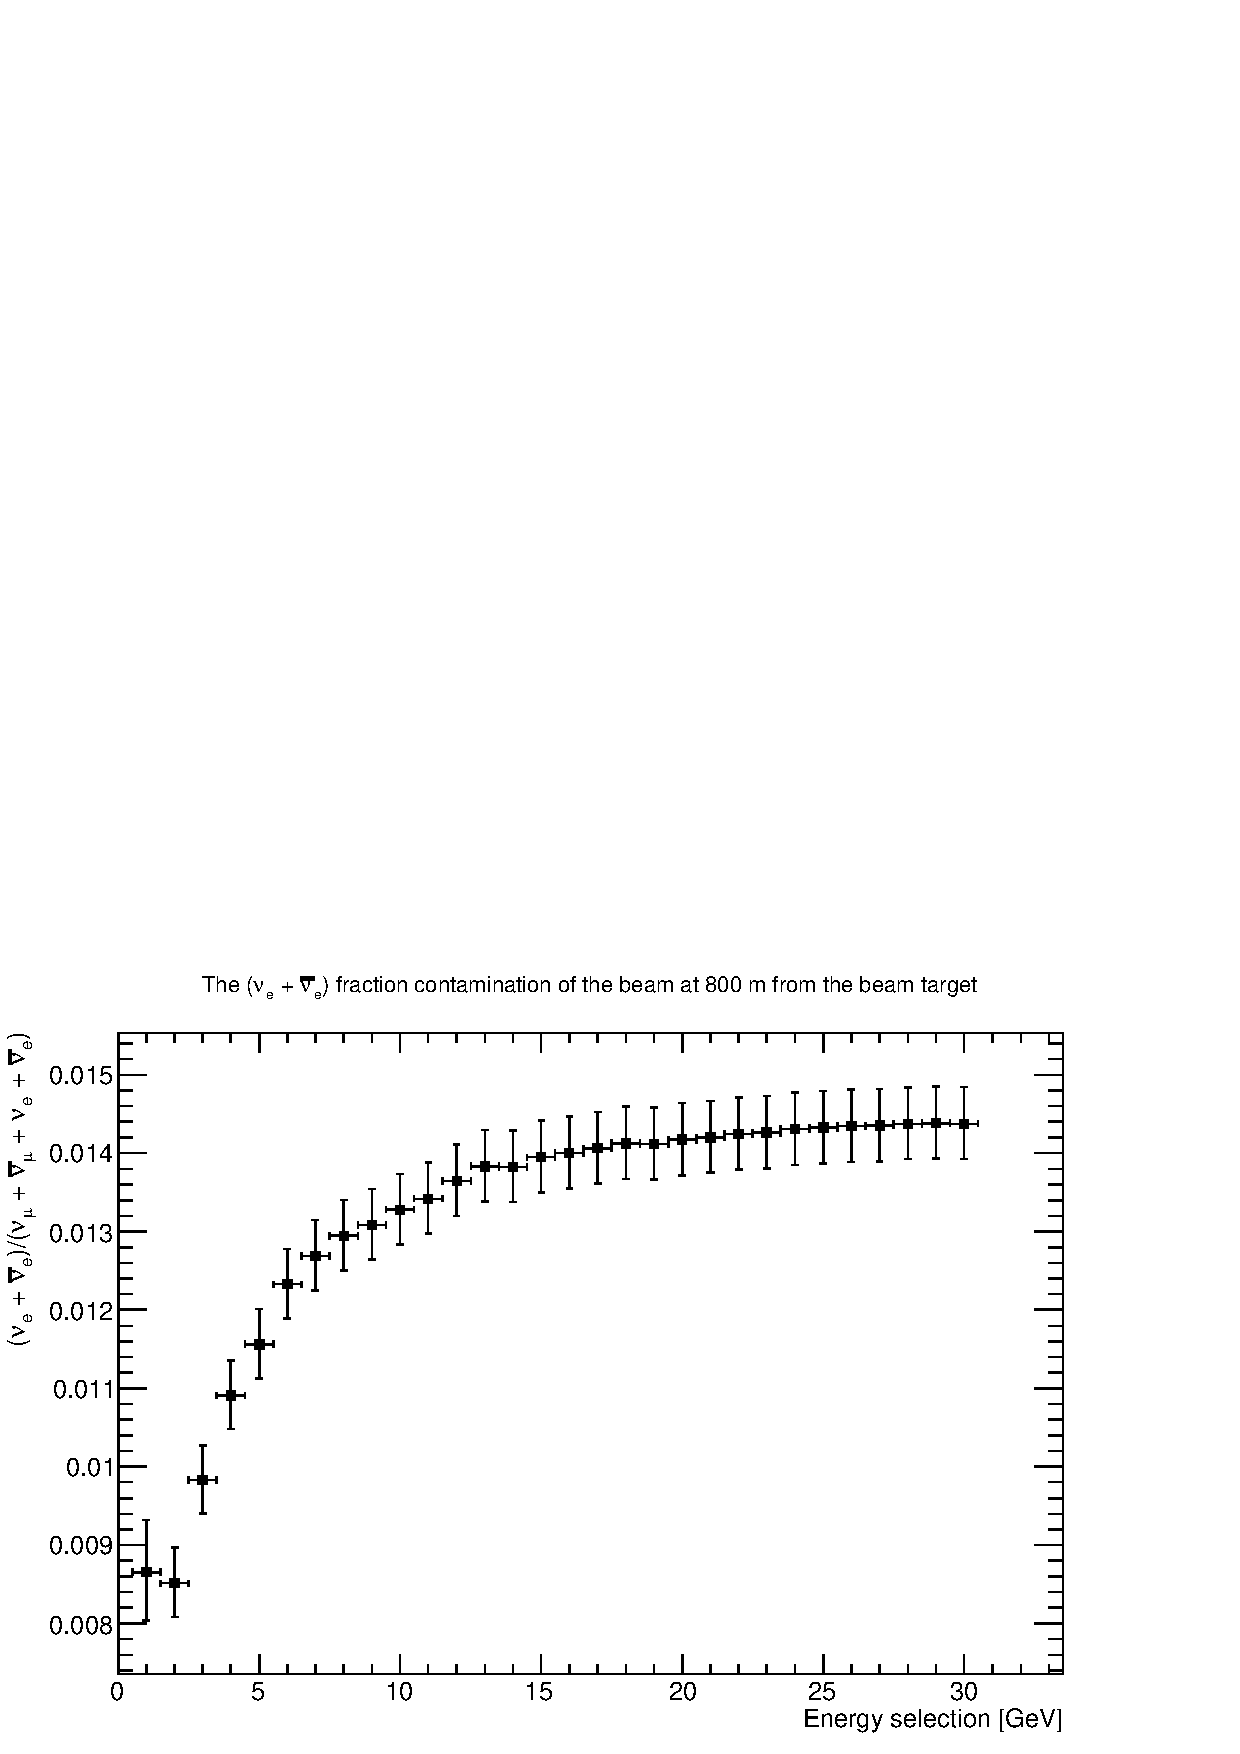
\includegraphics[width=120mm]{Chapter3/figures/400GeV_PF_nueAndNueBarRatio_EnergyCuts.pdf}
      \caption{The electron neutrino contamination, $\alpha_{\nu_{e}}^{cont}$ = ($\nu_{e}$ + $\bar{\nu}_{e}$)/($\nu_{\mu} + \bar{\nu}_{\mu} + \nu_{e} + \bar{\nu}_{e}$) for cumulative radius selections ranging from 1 to 30 m (top) and for cumulative energy selections from 1 to 30 GeV (bottom). No $\nu_{e}$ or $\bar{\nu}_{e}$ pass the radius selection for 1 m and hence no point is shown. Results based on 400 GeV positive focusing (PF) beam option only.}
    \label{fig:nueContamination}
\end{center}
\end{figure}

\begin{figure}[htbp]
\begin{center}
 	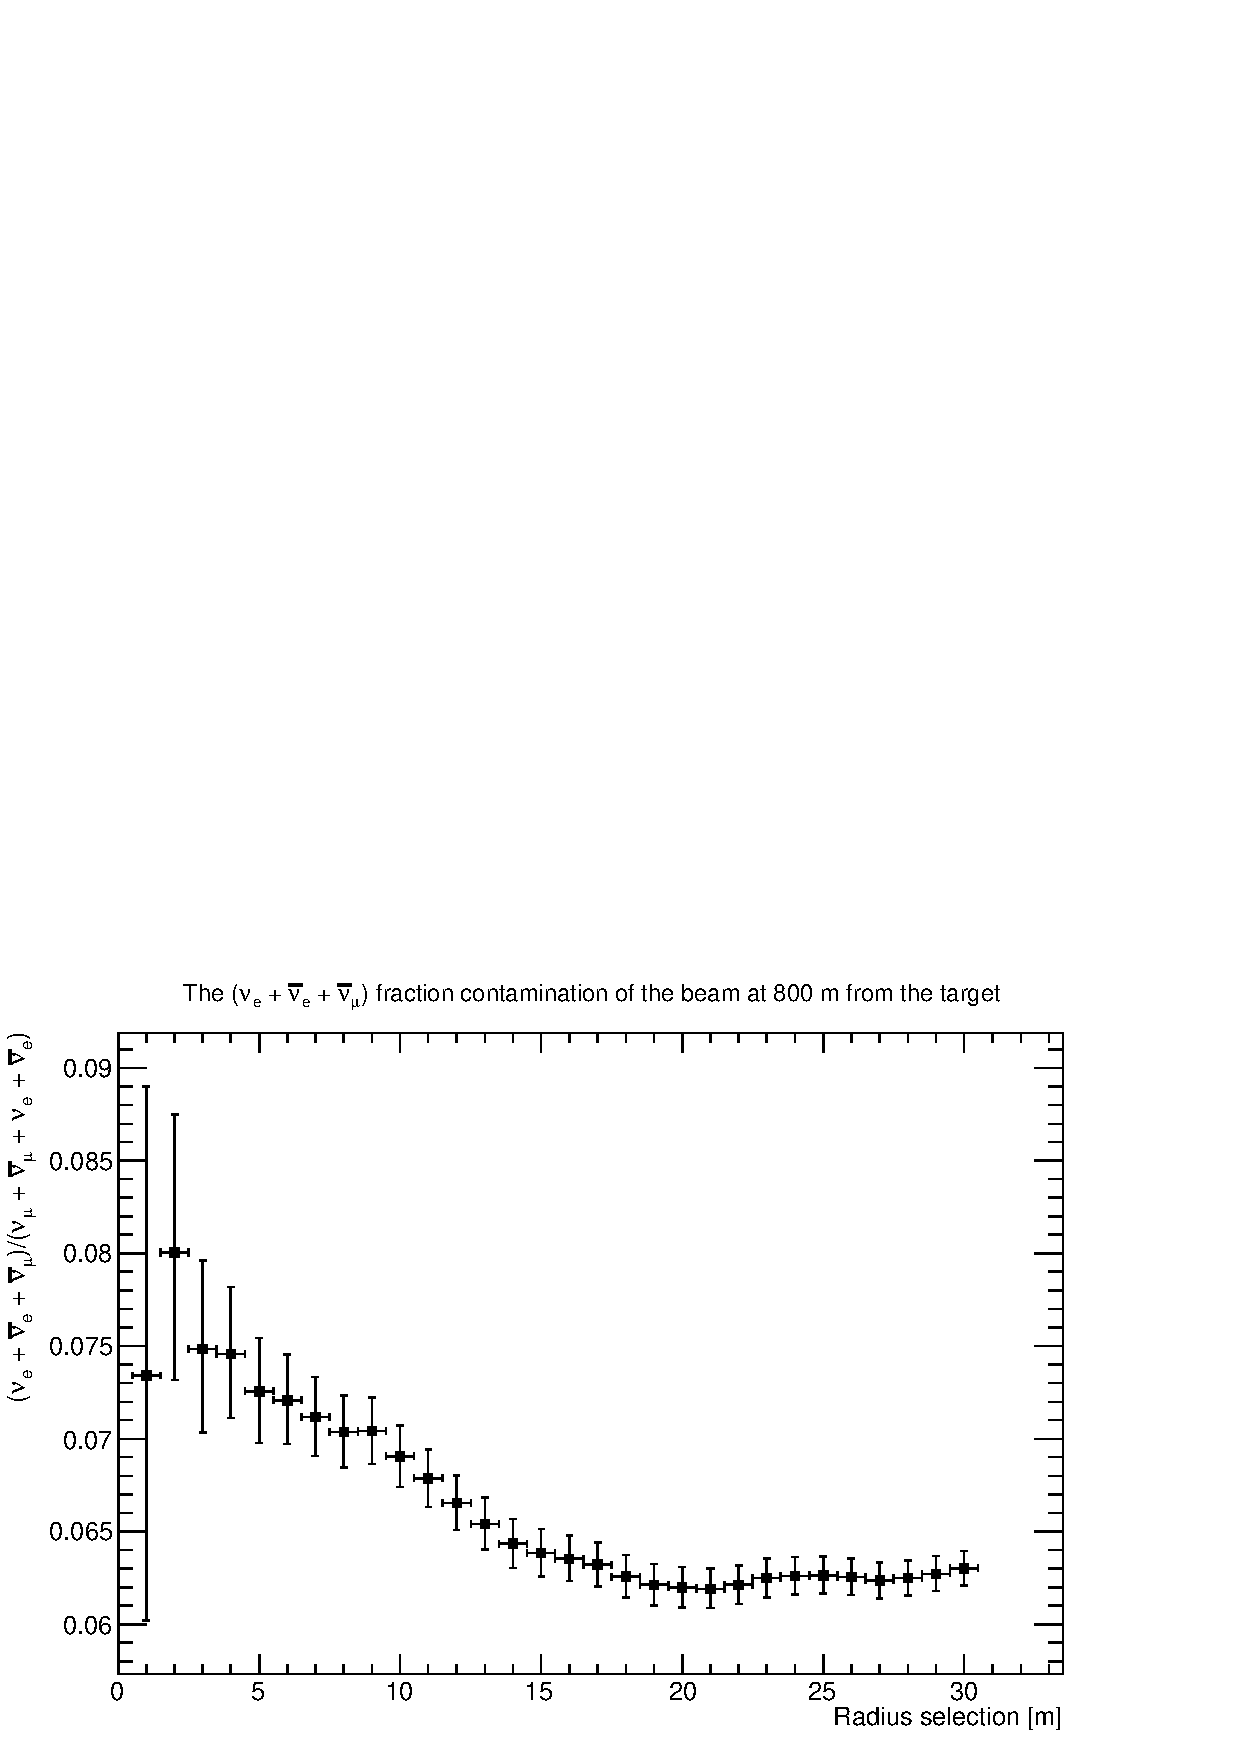
\includegraphics[width=120mm]{Chapter3/figures/400GeV_PF_nueAndNueBarAndNuMuBarRatio_RadiusCuts.pdf}
 	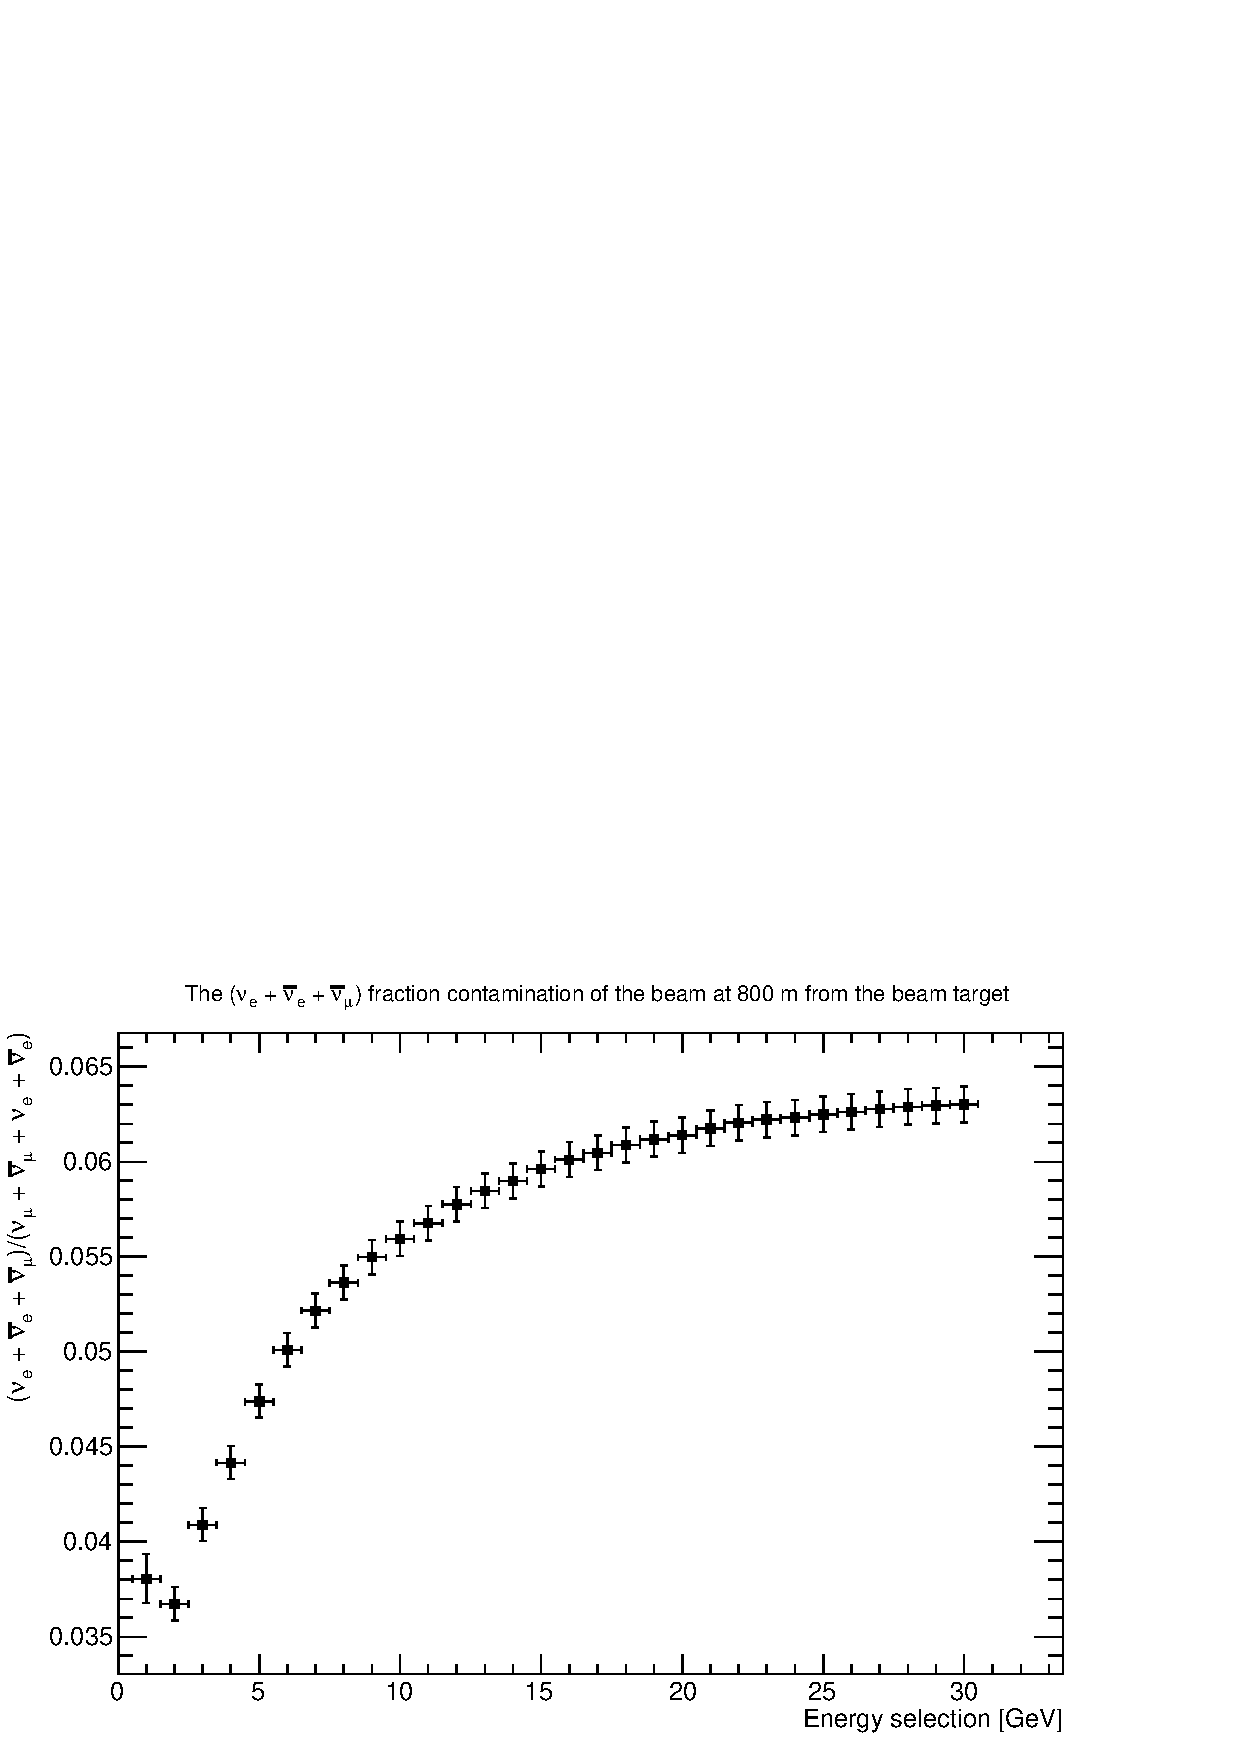
\includegraphics[width=120mm]{Chapter3/figures/400GeV_PF_nueAndNueBarAndNuMuBarRatio_EnergyCuts.pdf}
      \caption{The full neutrino contamination, $\alpha_{\nu_{e,\mu}}^{cont}$ = ($\nu_{e}$ + $\bar{\nu}_{e}$+ $\bar{\nu}_{\mu}$)/($\nu_{\mu} + \bar{\nu}_{\mu} + \nu_{e} + \bar{\nu}_{e}$) for cumulative radius selections ranging from 1 to 30 m (top) and for cumulative energy selections from 1 to 30 GeV (bottom). Results based on 400 GeV positive focusing (PF) beam option only.}
    \label{fig:nueAndNuMuBarContamination}
\end{center}
\end{figure}

\section{Prediction of Event Rates}
The neutrino event rate, $R_{\nu}$, at the detector can be estimated by equation \ref{eq:neutrinoEventRate}, which is summed over all neutrino flavours.
\begin{equation}
	R_{\nu} =  \frac{\rho V\epsilon}{m_{Ar}} \sum_{\alpha = \mu,e,\tau} \int_0^{E_{max}} \sigma^{TOT}_{\nu_{\alpha}}(E') \phi_{\nu_{\alpha}}(E') \hfill \mathrm{d}E'
	\label{eq:neutrinoEventRate}
\end{equation}
This equation is established assuming a 100\% argon detector with the a density $\rho$, efficiency $\epsilon$, total cross section (CC and NC) $\sigma^{TOT}_{\nu_{\alpha}}$ and flux $\phi_{\nu_{\alpha}}$, both as a function of neutrino energy. Where the total cross section for $\nu_{\mu}$ on $^{40}$Ar for CC and NC interactions is shown in figure \ref{fig:numuArgonCrossSection}. The mass of an argon atom is $m_{Ar}$ = 6.67 $\times$ 10$^{-26}$ kg.
\begin{figure}[hbtp]
	\begin{center}
		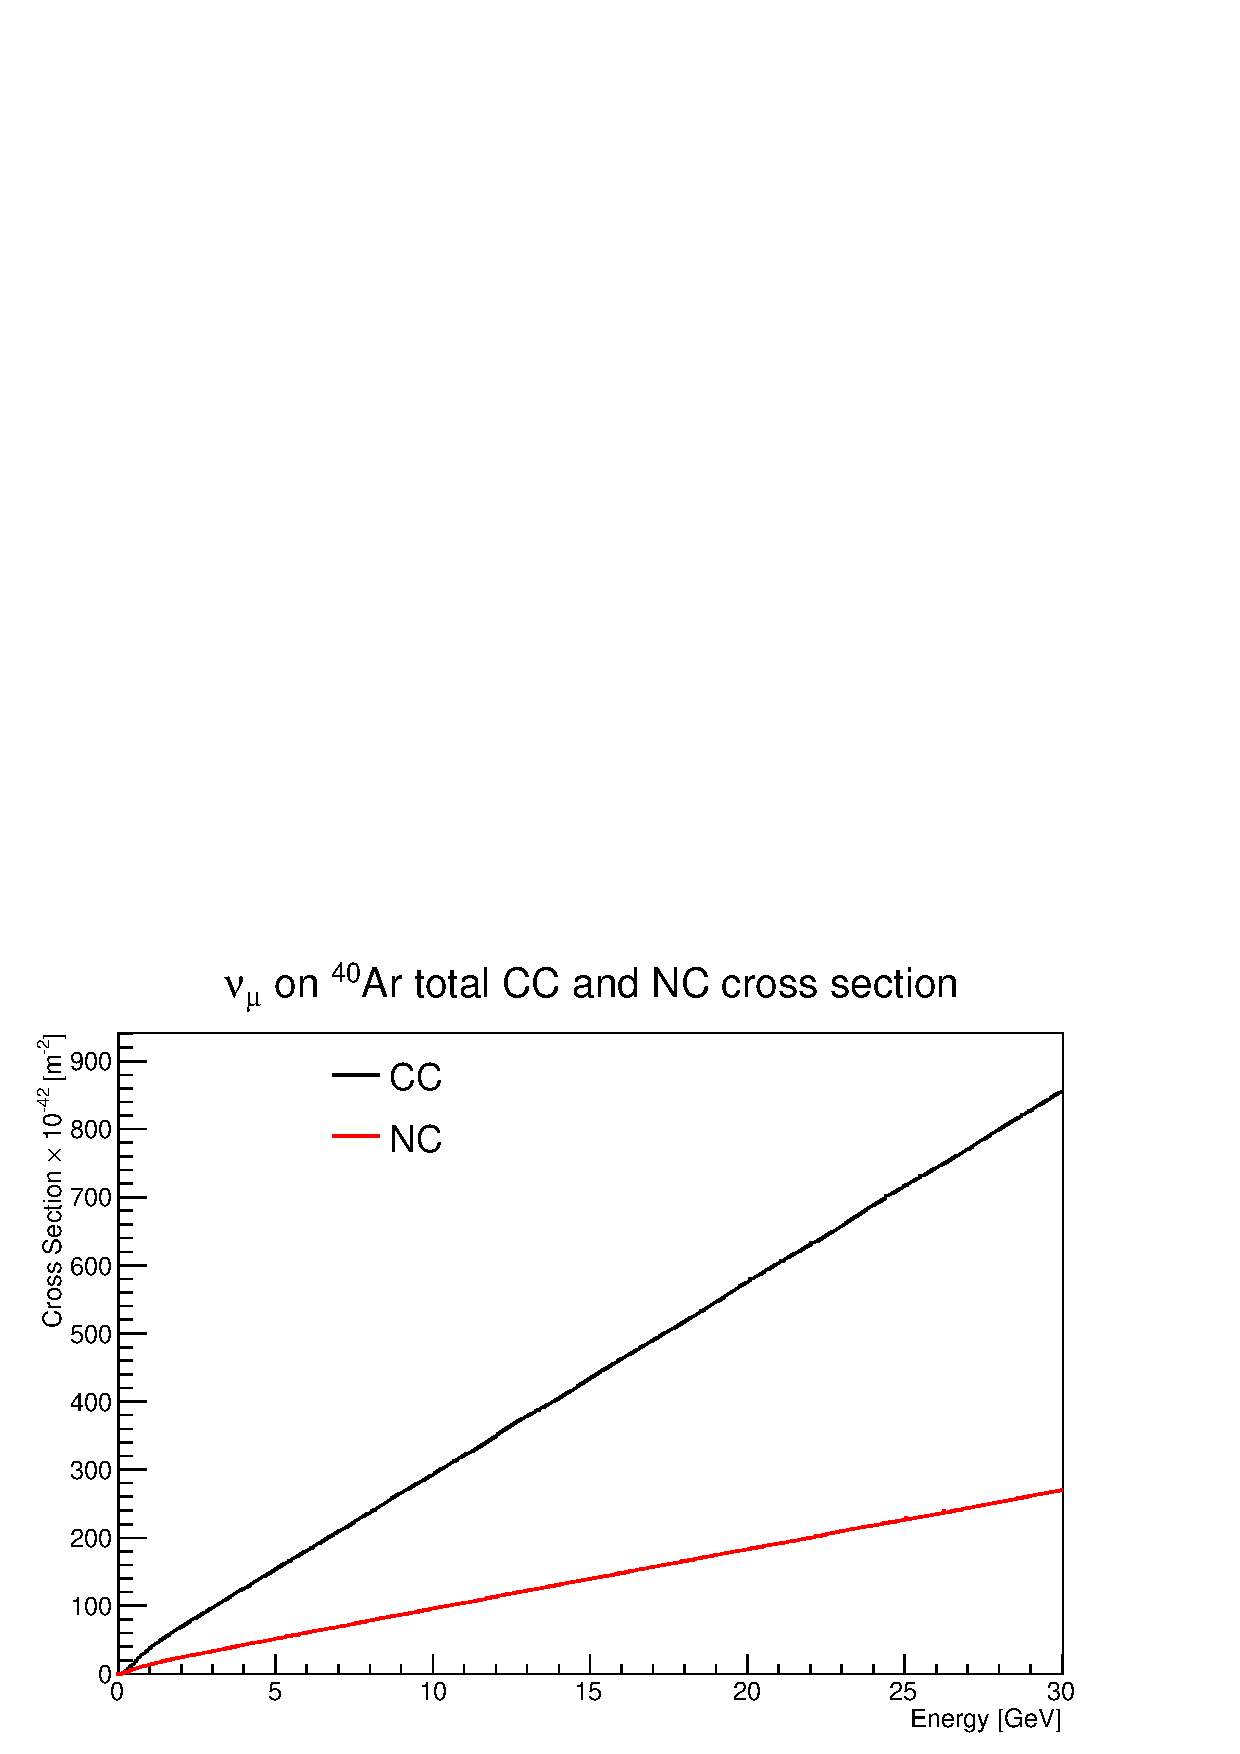
\includegraphics[width=100mm]{Chapter3/figures/numuAr40XSec_totalCCandNC.png}
	\caption{The muon neutrino CC and NC total cross sections on $^{40}$Ar for energies up to 30 GeV. The prediction is based on extrapolated data taken from the Monte Carlo generator GENIE 2.6.6 \cite{GENIE}. }
	\label{fig:numuArgonCrossSection}
\end{center}
\end{figure}

Multiplying the cross section with the neutrino flux on a binned basis and then summing each resultant bin gives an approximate estimate of the integral in equation \ref{eq:neutrinoEventRate}. Calculating rates for both LAr and GAr of volumes used in the ND, V = 8 m$^{3}$, with maximal efficiency are shown in table \ref{tab:gasAndLiquidArgonRates}, with various gas pressures and for both beam options.

\renewcommand{\arraystretch}{1.5}
\begin{table}
\begin{center}
  \begin{tabular}{l*{4}{c}r}
  \hline
  \textbf{State} &\textbf{Pressure} & \textbf{Temperature} & \textbf{Density} & \textbf{50 GeV} & \textbf{400 GeV} \\
  & & & & \textbf{beam rate} & \textbf{beam rate}\\
  \hline
  - & [MPa] & [k] & [kg m$^{-3}$] & [$\nu_{\mu}$ / 10$^{14}$ p.o.t] & [$\nu_{\mu}$ / 10$^{14}$ p.o.t] \\
  \hline
  \hline
  Liquid & - & 87.3 & 1400 & 4.61 $\pm$ 0.11 & 39.7 $\pm$ 2.5  \\
  Gas & 10.0 & 280 & 184 & 0.605 $\pm$ 0.014  & 5.22 $\pm$ 0.32  \\
  Gas & 5.0 & 280 & 89.3 & 0.294 $\pm$ 0.007  & 2.53 $\pm$ 0.16  \\
  Gas & 2.0 & 280 & 34.9 & 0.0115 $\pm$ 0.003  & 0.989 $\pm$ 0.061 \\
  Gas & 1.0 & 280 & 17.6 & 0.058 $\pm$ 0.001& 0.499 $\pm$ 0.031\\
  Gas & 0.5 & 280 & 8.7 & 0.029 $\pm$ 0.001 & 0.247 $\pm$ 0.015  \\
    \hline
  \end{tabular}
      \caption{Estimated $\nu_{\mu}$ rates using equation \ref{eq:neutrinoEventRate} for a ND of 2 $\times$ 2 $\times$ 2 m$^{3}$ at 800m from the target. Uncertainties relate to 1$\sigma$ statistical errors propagating from neutrino flux estimation only, other parameters are assumed to have negligible errors. Densities and pressures for argon taken from \cite{argonDensities}.}
    \label{tab:gasAndLiquidArgonRates}
\end{center}
    \end{table}
\renewcommand{\arraystretch}{1.0}

\section{Detector Concept}
The basic design of the ND, omitting the magnet is shown by an artists impression in figure \ref{fig:ndDesign}.

\begin{figure}[hbtp]
	\begin{center}
		\includegraphics[width=49mm]{Chapter3/figures/8_LBNO2.png}
		\includegraphics[width=49mm]{Chapter3/figures/9_LBNO1.png}
		\includegraphics[width=50mm]{Chapter3/figures/5_LBNO5.png}
	\caption{A graphical representation of the current ND design, showing the pressure vessel (left), scintillator bars/layers (middle) and the TPC (right). The magnet is omitted from this sketch.}
	\label{fig:ndLayers}
	\end{center}
\end{figure}

\begin{figure}[htbp]
	\begin{center}
		\includegraphics[width=100mm]{Chapter3/figures/1_LBNO3.pdf}
		\caption{A graphical interpretation of the current ND design for the proposed LAGUNA-LBNO experiment. The magnet is omitted from this sketch.}
		\label{fig:ndDesign}
	\end{center}
\end{figure}

